\documentclass[12pt,a4paper]{article}

% Packages
\usepackage{geometry}
\geometry{margin=1in}
\usepackage{fancyhdr}
\usepackage{titlesec}
\usepackage{listings}
\usepackage{xcolor}
\usepackage{graphicx} 

% Header & Footer
\pagestyle{fancy}
\fancyhf{}
\rhead{C++ - Assignment 4}
\lhead{Kamithkar Vinod}
\cfoot{\thepage}

% Title formatting
\titleformat{\section}{\large\bfseries}{Problem \thesection:}{0.5em}{}
\titleformat{\subsection}[runin]{\bfseries}{Code:}{0.5em}{}[---]
\titleformat{\subsubsection}[runin]{\bfseries}{Output:}{0.5em}{}[---]

% Code style
\lstset{
    language=cpp,
    basicstyle=\ttfamily\small,
    keywordstyle=\color{blue}\bfseries,
    commentstyle=\color{gray}\itshape,
    stringstyle=\color{red},
    showstringspaces=false,
    numbers=left,
    numberstyle=\tiny\color{gray},
    frame=single,
    breaklines=true
}

% Document Start
\begin{document}

% Title Page
\begin{center}
    \LARGE \textbf{Assignment - 4} \\[0.5cm]
    \Large \textbf{C++} \\[1cm]

    \begin{tabular}{rl}
        \textbf{Name:} & Kamithkar Vinod \\
        \textbf{Course:} & PG DAC AUGUST 2025 \\
        \textbf{PRN:} & 250850320040 \\
        \textbf{Form No:} & 250500480 \\
        \textbf{Date:} & 09-10-2025 \\
    \end{tabular}
\end{center}

\vspace{1cm}
\hrule
\vspace{0.5cm}

% Problems
% 1
\section{Smart Inventory System with Dynamic Memory and Inheritance}
\textbf{Task:} Design a program to manage an inventory system for a store.
Each item in the store belongs to a specific category (like Electronics or Groceries), but the data must be stored and managed without using virtual functions.
You must handle object relationships, memory allocation, and cleanup properly.


\subsection{}
\begin{lstlisting}
#include <iostream>
#include <string>
#include <vector>
#include <iomanip>

using namespace std;

// ItemType helps us manage pointer-to-object relationships without virtual functions.
enum class ItemType {
    BASE,
    ELECTRONICS,
    GROCERIES
};

// ----------------------
// Base Class: Item
// ----------------------
class Item {
private:
    string name;
    int id;
    float price;

protected:
    int quantity;
    ItemType type; // store the actual runtime type (set by derived classes)

public:
    // Parameterized constructor
    Item(const string& name_, int id_, float price_, int quantity_)
        : name(name_), id(id_), price(price_), quantity(quantity_), type(ItemType::BASE) {
    }

    // Display base item details
    void display() const {
        cout << left << setw(15) << name
             << setw(8) << id
             << setw(10) << fixed << setprecision(2) << price
             << setw(10) << quantity;
    }

    // Return total value: price * quantity
    float getTotalValue() const {
        return price * quantity;
    }

    // Accessors
    string getName() const { return name; }
    int getId() const { return id; }
    float getPrice() const { return price; }
    ItemType getType() const { return type; }

    // Destructor (non-virtual by requirement)
    ~Item() {
        cout << "Destroying Item (id=" << id << ", name=\"" << name << "\")\n";
    }
};

// ----------------------
// Derived Class: Electronics
// ----------------------
class Electronics : public Item {
private:
    int warrantyMonths; // additional member

public:
    Electronics(const string& name_, int id_, float price_, int quantity_, int warrantyMonths_)
        : Item(name_, id_, price_, quantity_), warrantyMonths(warrantyMonths_) {
        // mark derived type
        // Access protected member 'type' from base class
        type = ItemType::ELECTRONICS;
    }

    void display() const {
        // Call base display for common fields
        Item::display();
        cout << setw(15) << warrantyMonths << endl;
    }

    int getWarranty() const { return warrantyMonths; }

    ~Electronics() {
        cout << "Destroying Electronics specific resources (id=" << getId() << ")\n";
    }
};

// ----------------------
// Derived Class: Groceries
// ----------------------
class Groceries : public Item {
private:
    string expiryDate; // example: "2025-12-31"

public:
    Groceries(const string& name_, int id_, float price_, int quantity_, const string& expiryDate_)
        : Item(name_, id_, price_, quantity_), expiryDate(expiryDate_) {
        type = ItemType::GROCERIES;
    }

    void display() const {
        Item::display();
        cout << setw(15) << expiryDate << endl;
    }

    string getExpiry() const { return expiryDate; }

    ~Groceries() {
        cout << "Destroying Groceries specific resources (id=" << getId() << ")\n";
    }
};

// ----------------------
// Helper: print header
// ----------------------
void printInventoryHeader() {
    cout << left << setw(15) << "Name" << setw(8) << "ID" << setw(10) << "Price" << setw(10) << "Qty";
    cout << setw(15) << "Extra" << endl;
    cout << string(58, '-') << endl;
}

// ----------------------
// Main demo
// ----------------------
int main() {
    // We'll keep pointers to base class but store runtime type in each object.
    vector<Item*> items;

    // Dynamically allocate different derived objects
    items.push_back(new Electronics("SmartPhone", 101, 19999.00f, 5, 24));    // warranty 24 months
    items.push_back(new Groceries("Rice", 201, 59.50f, 50, "2026-01-15"));    // expiry
    items.push_back(new Electronics("Laptop", 102, 55999.99f, 2, 12));
    items.push_back(new Groceries("Milk", 202, 45.00f, 30, "2025-10-20"));

    // Display inventory
    cout << "\nCurrent Inventory:\n";
    printInventoryHeader();
    for (const Item* it : items) {
        if (it->getType() == ItemType::ELECTRONICS) {
            // safe because we know actual type via stored enum
            const Electronics* e = static_cast<const Electronics*>(it);
            e->display();
        } else if (it->getType() == ItemType::GROCERIES) {
            const Groceries* g = static_cast<const Groceries*>(it);
            g->display();
        } else {
            // base-only item
            it->display();
            cout << endl;
        }
    }

    // Compute and print total inventory value
    float grandTotal = 0.0f;
    for (const Item* it : items) {
        grandTotal += it->getTotalValue();
    }
    cout << "\nGrand Total Value of Inventory: INR " << fixed << setprecision(2) << grandTotal << "\n";

    // Proper cleanup: delete via the actual derived type pointer.
    // IMPORTANT: since base destructor is NOT virtual, do NOT delete using 'delete items[i]' when
    // items[i] is typed Item* and actually points to a derived object. We instead cast to derived
    // pointer type and delete via that pointer.
    cout << "\nCleaning up dynamically allocated objects:\n";
    for (Item* it : items) {
        ItemType t = it->getType();
        if (t == ItemType::ELECTRONICS) {
            Electronics* e = static_cast<Electronics*>(it);
            delete e; // deletes derived then base destructor
        } else if (t == ItemType::GROCERIES) {
            Groceries* g = static_cast<Groceries*>(it);
            delete g;
        } else {
            // If there were plain Item objects allocated directly, we'd delete them like this:
            delete it;
        }
    }

    items.clear();
    cout << "All objects cleaned up.\n";

    return 0;
}


\end{lstlisting}

\subsubsection{1}
\begin{center}
    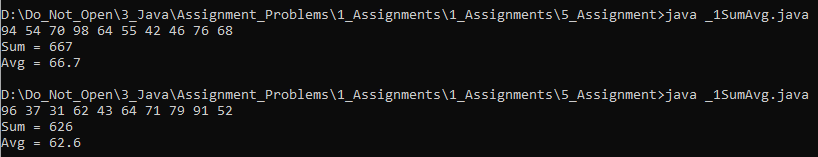
\includegraphics[width=0.8\textwidth]{1.png}
\end{center}


% 2

\section{Employee Payroll Management System (with Dynamic Bonus Calculation))}
\textbf{Task:} Design a C++ program to manage employees of a company.
Each employee has common details (name, ID, base salary), but different roles (e.g.,Manager, Developer) that determine their bonus.
You must use classes, inheritance, encapsulation, constructors, destructors, and pointers to:
    \item - ● Store and display employee information.
    \item - ● Dynamically allocate memory for employees.

    \item - ● Compute their total salary (base + bonus).
    \item - ● Ensure proper cleanup of allocated memory.
\subsection{}
\begin{lstlisting}
#include <iostream>
#include <string>
#include <iomanip>
using namespace std;

// ============================
// Base Class: Employee
// ============================
class Employee {
private:
    string name;
    int id;
    float baseSalary;

protected:
    float bonus;

public:
    // Parameterized Constructor
    Employee(const string& name_, int id_, float baseSalary_)
        : name(name_), id(id_), baseSalary(baseSalary_), bonus(0.0f) {}

    // Virtual Function - Base version
    virtual void calculateBonus() {
        bonus = 0.0f;  // Base class: no bonus
    }

    // Virtual Display Function
    virtual void display() const {
        cout << left << setw(15) << name
             << setw(8) << id
             << setw(12) << fixed << setprecision(2) << baseSalary
             << setw(12) << bonus
             << setw(15) << "Employee"
             << setw(12) << baseSalary + bonus
             << endl;
    }

    // Virtual Destructor
    virtual ~Employee() {
        cout << "Destroying Employee object: " << id << " (" << name << ")\n";
    }

protected:
    // Protected getters for derived class access
    string getName() const { return name; }
    int getId() const { return id; }
    float getBaseSalary() const { return baseSalary; }
};

// ============================
// Derived Class: Manager
// ============================
class Manager : public Employee {
public:
    Manager(const string& name_, int id_, float baseSalary_)
        : Employee(name_, id_, baseSalary_) {}

    void calculateBonus() override {
        bonus = 0.40f * getBaseSalary();  // 40% of base salary
    }

    void display() const override {
        cout << left << setw(15) << getName()
             << setw(8) << getId()
             << setw(12) << fixed << setprecision(2) << getBaseSalary()
             << setw(12) << bonus
             << setw(15) << "Manager"
             << setw(12) << getBaseSalary() + bonus
             << endl;
    }

    ~Manager() override {
        cout << "Destroying Manager object: " << getId() << "\n";
    }
};

// ============================
// Derived Class: Developer
// ============================
class Developer : public Employee {
public:
    Developer(const string& name_, int id_, float baseSalary_)
        : Employee(name_, id_, baseSalary_) {}

    void calculateBonus() override {
        bonus = 0.25f * getBaseSalary();  // 25% of base salary
    }

    void display() const override {
        cout << left << setw(15) << getName()
             << setw(8) << getId()
             << setw(12) << fixed << setprecision(2) << getBaseSalary()
             << setw(12) << bonus
             << setw(15) << "Developer"
             << setw(12) << getBaseSalary() + bonus
             << endl;
    }

    ~Developer() override {
        cout << "Destroying Developer object: " << getId() << "\n";
    }
};

// ============================
// Helper Function: Header
// ============================
void printHeader() {
    cout << left
         << setw(15) << "Name"
         << setw(8)  << "ID"
         << setw(12) << "BaseSalary"
         << setw(12) << "Bonus"
         << setw(15) << "Role"
         << setw(12) << "TotalSalary"
         << endl;
    cout << string(74, '-') << endl;
}

// ============================
// Main Function
// ============================
int main() {
    int n;
    cout << "Enter the number of employees: ";
    cin >> n;

    Employee** employees = new Employee*[n]; // Array of base pointers

    for (int i = 0; i < n; ++i) {
        cout << "\nEnter details for employee #" << i + 1 << ":\n";

        string name;
        int id, choice;
        float salary;

        cout << "Name: ";
        cin >> ws;
        getline(cin, name);
        cout << "ID: ";
        cin >> id;
        cout << "Base Salary: ";
        cin >> salary;

        cout << "Select Role (1 - Manager, 2 - Developer): ";
        cin >> choice;

        if (choice == 1)
            employees[i] = new Manager(name, id, salary);
        else
            employees[i] = new Developer(name, id, salary);

        // Calculate bonus for each employee
        employees[i]->calculateBonus();
    }

    // Display all employee details
    cout << "\n\nEmployee Payroll Details:\n";
    printHeader();
    for (int i = 0; i < n; ++i) {
        employees[i]->display();
    }

    // Cleanup
    cout << "\nCleaning up memory:\n";
    for (int i = 0; i < n; ++i) {
        delete employees[i];
    }
    delete[] employees;

    cout << "All employee objects destroyed successfully.\n";
    return 0;
}


\end{lstlisting}

\subsubsection{}
\begin{center}
    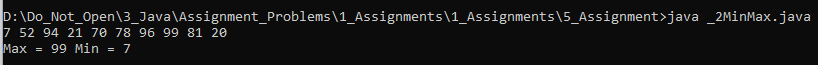
\includegraphics[width=0.8\textwidth]{2.png}
\end{center}

% 3

\section{Menu-Driven Employee Management System using Classes, Objects, Inheritance, and Dynamic Memory in C++}
\textbf{Task:} Design a Menu-Driven Employee Management System for a company that manages two types of employees:
1. FullTimeEmployee

2. PartTimeEmployee

You must:
● Use inheritance to derive these two classes from a base class Employee.
● Use encapsulation for data hiding (private/protected members).
● Create objects dynamically using pointers.
● Display and manage data using a menu-driven interface.

\subsection{}
\begin{lstlisting}
#include <iostream>
#include <string>
#include <vector>
#include <iomanip>
using namespace std;

// ======================================
// Base Class: Employee
// ======================================
class Employee {
private:
    string name;
    int empID;

protected:
    float salary;

public:
    // Parameterized constructor
    Employee(const string& name_, int empID_)
        : name(name_), empID(empID_), salary(0.0f) {}

    // Display basic info
    void displayBasic() const {
        cout << left << setw(15) << name
             << setw(10) << empID;
    }

    // Getter
    float getSalary() const { return salary; }

    int getID() const { return empID; }
    string getName() const { return name; }

    // Virtual destructor
    virtual ~Employee() {
        cout << "Destroying Employee: " << empID << " (" << name << ")\n";
    }

    // Virtual functions to override
    virtual void calculateSalary() = 0;
    virtual void displayDetails() const = 0;
};

// ======================================
// Derived Class: FullTimeEmployee
// ======================================
class FullTimeEmployee : public Employee {
private:
    float basicPay;
    float bonus;

public:
    FullTimeEmployee(const string& name_, int empID_, float basicPay_, float bonus_)
        : Employee(name_, empID_), basicPay(basicPay_), bonus(bonus_) {}

    void calculateSalary() override {
        salary = basicPay + bonus;
    }

    void displayDetails() const override {
        displayBasic();
        cout << setw(15) << "Full-Time"
             << setw(12) << fixed << setprecision(2) << salary
             << setw(12) << basicPay
             << setw(12) << bonus
             << endl;
    }

    ~FullTimeEmployee() override {
        cout << "Cleaning up FullTimeEmployee object (ID=" << getID() << ")\n";
    }
};

// ======================================
// Derived Class: PartTimeEmployee
// ======================================
class PartTimeEmployee : public Employee {
private:
    int hoursWorked;
    float hourlyRate;

public:
    PartTimeEmployee(const string& name_, int empID_, int hoursWorked_, float hourlyRate_)
        : Employee(name_, empID_), hoursWorked(hoursWorked_), hourlyRate(hourlyRate_) {}

    void calculateSalary() override {
        salary = hoursWorked * hourlyRate;
    }

    void displayDetails() const override {
        displayBasic();
        cout << setw(15) << "Part-Time"
             << setw(12) << fixed << setprecision(2) << salary
             << setw(12) << hoursWorked
             << setw(12) << hourlyRate
             << endl;
    }

    ~PartTimeEmployee() override {
        cout << "Cleaning up PartTimeEmployee object (ID=" << getID() << ")\n";
    }
};

// ======================================
// Helper Function: Display Header
// ======================================
void displayHeader() {
    cout << left << setw(15) << "Name"
         << setw(10) << "EmpID"
         << setw(15) << "Type"
         << setw(12) << "Salary"
         << setw(12) << "Basic/Hrs"
         << setw(12) << "Bonus/Rate"
         << endl;
    cout << string(76, '-') << endl;
}

// ======================================
// Search Function
// ======================================
Employee* searchEmployee(vector<Employee*>& employees, int id) {
    for (auto* e : employees) {
        if (e->getID() == id)
            return e;
    }
    return nullptr;
}

// ======================================
// Delete Function
// ======================================
void deleteEmployee(vector<Employee*>& employees, int id) {
    for (auto it = employees.begin(); it != employees.end(); ++it) {
        if ((*it)->getID() == id) {
            delete *it; // Free memory
            employees.erase(it);
            cout << "Employee with ID " << id << " deleted successfully.\n";
            return;
        }
    }
    cout << "Employee with ID " << id << " not found.\n";
}

// ======================================
// Main Function
// ======================================
int main() {
    vector<Employee*> employees;
    int choice;

    do {
        cout << "\n=========== Employee Management System ===========\n";
        cout << "1. Add Full-Time Employee\n";
        cout << "2. Add Part-Time Employee\n";
        cout << "3. Display All Employees\n";
        cout << "4. Search Employee by ID\n";
        cout << "5. Delete Employee by ID\n";
        cout << "6. Exit\n";
        cout << "Enter your choice: ";
        cin >> choice;

        switch (choice) {
        case 1: {
            string name;
            int id;
            float basic, bonus;
            cout << "Enter name: ";
            cin >> ws;
            getline(cin, name);
            cout << "Enter ID: ";
            cin >> id;
            cout << "Enter Basic Pay: ";
            cin >> basic;
            cout << "Enter Bonus: ";
            cin >> bonus;

            Employee* e = new FullTimeEmployee(name, id, basic, bonus);
            e->calculateSalary();
            employees.push_back(e);
            cout << "Full-Time Employee added successfully!\n";
            break;
        }

        case 2: {
            string name;
            int id, hours;
            float rate;
            cout << "Enter name: ";
            cin >> ws;
            getline(cin, name);
            cout << "Enter ID: ";
            cin >> id;
            cout << "Enter Hours Worked: ";
            cin >> hours;
            cout << "Enter Hourly Rate: ";
            cin >> rate;

            Employee* e = new PartTimeEmployee(name, id, hours, rate);
            e->calculateSalary();
            employees.push_back(e);
            cout << "Part-Time Employee added successfully!\n";
            break;
        }

        case 3: {
            if (employees.empty()) {
                cout << "No employees to display.\n";
            } else {
                displayHeader();
                for (auto* e : employees)
                    e->displayDetails();
            }
            break;
        }

        case 4: {
            int id;
            cout << "Enter Employee ID to search: ";
            cin >> id;
            Employee* emp = searchEmployee(employees, id);
            if (emp) {
                displayHeader();
                emp->displayDetails();
            } else {
                cout << "Employee not found.\n";
            }
            break;
        }

        case 5: {
            int id;
            cout << "Enter Employee ID to delete: ";
            cin >> id;
            deleteEmployee(employees, id);
            break;
        }

        case 6: {
            cout << "Exiting program...\n";
            break;
        }

        default:
            cout << "Invalid choice. Please try again.\n";
        }

    } while (choice != 6);

    // Cleanup before exit
    cout << "\nCleaning up all remaining employee objects...\n";
    for (auto* e : employees)
        delete e;
    employees.clear();

    cout << "All memory released successfully.\n";
    return 0;
}

\end{lstlisting}

\subsubsection{}
\begin{center}
    \includegraphics[width=0.8\textwidth]{3_1.png}
\end{center}

\begin{center}
    \includegraphics[width=0.8\textwidth]{3_2.png}
\end{center}



\end{document}



